Испытания представляют собой процесс установления соответствия программы и
программной документации заданным требованиям.

\subsubsection{Проверка требований к документации}
Проверяеться наличие всех документов перечисленных в пyнкте 4.1 данного документа и их соответствие ГОСТ.

\subsection{Проверка требований к интерфейсу}
Интерфейс соответствует схеме, указанной в техническом задании, обладает шкалой времени, панелью для отображения иерархии, панелью для изменения настроек программы и панелью для отрисовки трехмерных элементов.

\begin{figure}[h!]
    \centering
    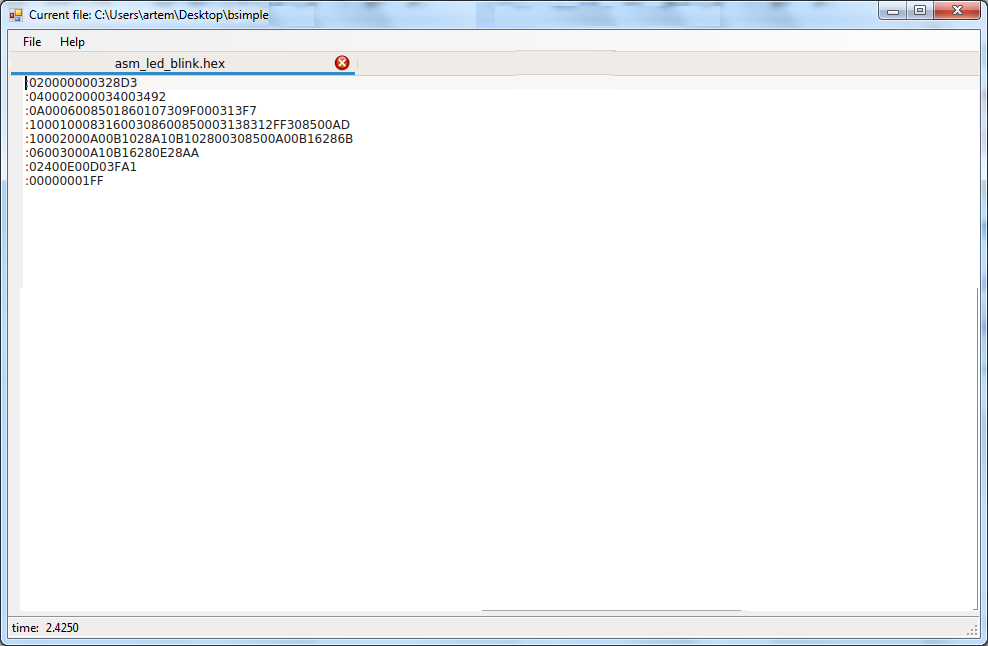
\includegraphics[width=0.5\textwidth]{../screenshots/interface_map.png}
    \caption{Изображение интерфейса программы}
\end{figure}

Дополние панели также удовлетворяют требованиям ТЗ:
\begin{figure}
\centering
\begin{minipage}{.4\textwidth}
  \centering
  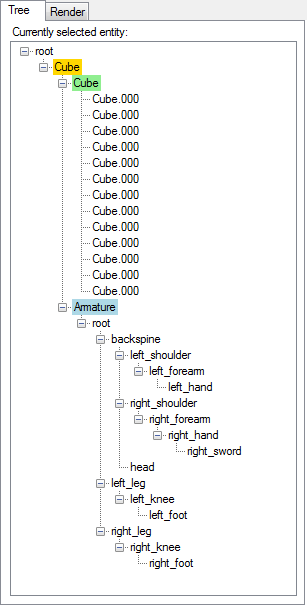
\includegraphics[height=.2\textheight]{../screenshots/tree_view_panel.png}
  \captionof{figure}{Панель отображения иерархии костей}
\end{minipage}%
\begin{minipage}{.4\textwidth}
  \centering
  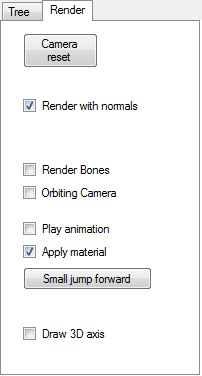
\includegraphics[height=.2\textheight]{../screenshots/render_panel.png}
  \captionof{figure}{Панель настройки программы}
\end{minipage}
\end{figure}

\subsection{Проверка требований к функциональным характеристикам}
Для загрузки данных из формата коллада (collada или .dae) необходимо выбрать его либо в меню "Open Recent", либо в меню "Open":

\begin{figure}[h!]
    \centering
    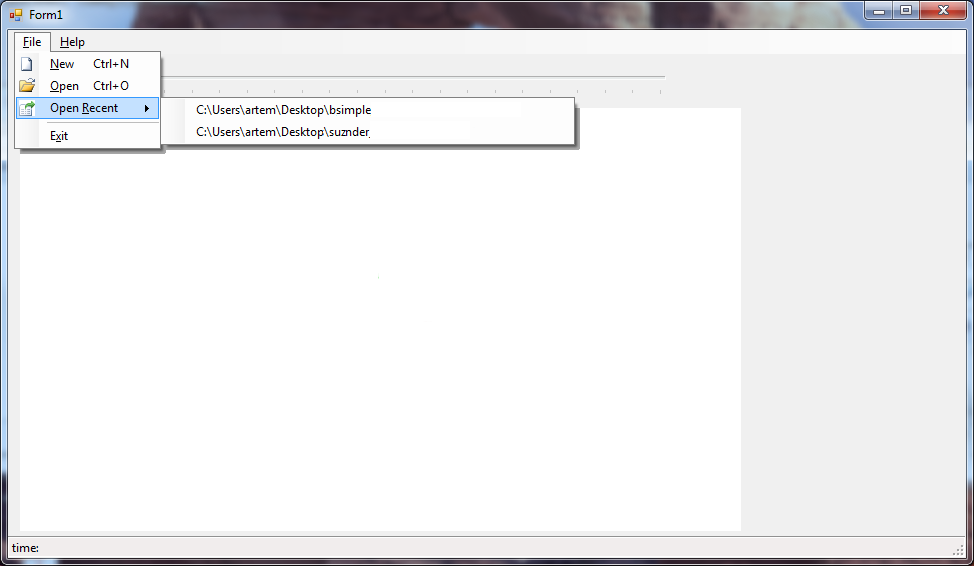
\includegraphics[width=0.8\textwidth]{../screenshots/file_menu_with_recent.png}
    \caption{Загрузка файла}
\end{figure}

Откроется диалог выбора файла:
\begin{figure}[h!]
    \centering
    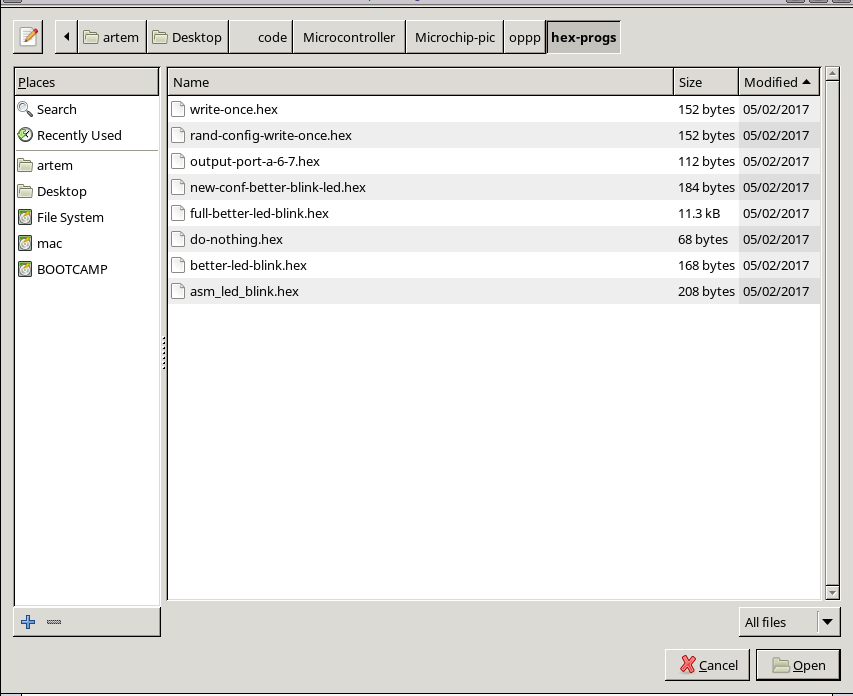
\includegraphics[width=0.5\textwidth]{../screenshots/open_file_dialog.png}
    \caption{Диалог выбора файла}
\end{figure}

После загрузки файла видно что его имя добавилось в список недавно открытых файлов "Recent Files".


%=================
У пользователя имеется возможность изменять ракурс и приближение камеры при помощи мышки. Структура загруженных данных отображена в виде дерева на панели справа. Также выделенная кость подсвеченна ярко-синим цветом.

\begin{figure}[h!]
    \centering
    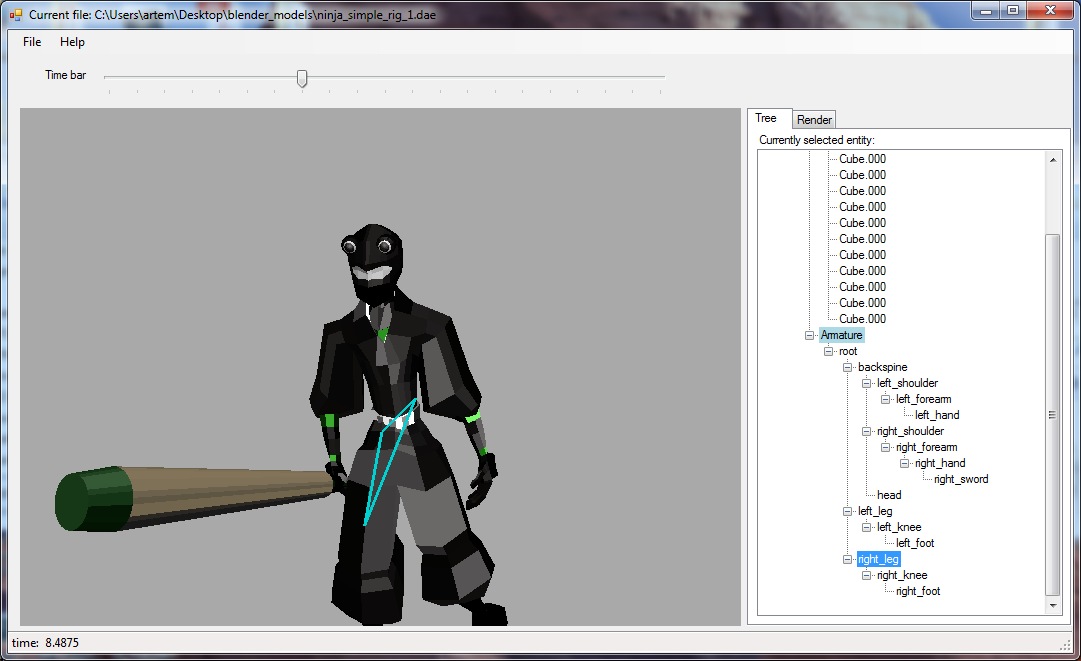
\includegraphics[width=0.8\textwidth]{../screenshots/frame_with_one_bone.png}
    \caption{Подсветка выбранной кости}
\end{figure}

Также есть панель для настоек работы программы позволяющая изменять следующие параметры:
\begin{my_enumerate}
\item Выбор между двумя видами камер в OpenGL, первый вид это камера движение которой сковано орбитой вокруг модели и другой тип это камера двигающаяся совершенно свободно.
\item Воспроизведение анимации.
\item Включение и выключение отрисовки с учетом нормалей.
\item Включение и выключение отрисовки с учетом характеристик материала.
\item Отрисовка всех костей скелета.
\end{my_enumerate}

%=================
Элемент ScrollBar показывает текущий момент в анимации и предоставляет 
возможность перейти к любому моменту времени. 

\begin{figure}[h!]
    \centering
    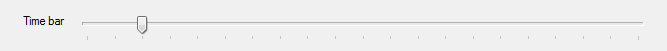
\includegraphics[width=0.5\textwidth]{../screenshots/time_bar.png}
    \caption{Элемент ScrollBar}
\end{figure}

\bigskip

Поддерживатся изменение размеров окна приложения, без изменения соотношения проекции OpenGL.


\subsection{Проверка требований к надежности}
Оператор должен воспользоваться всеми функциями программы и убедиться, что они не приводят к ее аварийному завершению.
